%======================================================================
\begin{abstract}
We present \name, a fully automatic system that converts posed RGB images
of a real indoor scene---together with its reconstruction as a mesh and a
Gaussian splat---into an editable, photorealistic, simulation-ready
digital twin, without any semantic annotations or user interaction. Every
object except the building shell is (i)~discovered by lifting
open-vocabulary 2D masks onto the scene mesh with occlusion-aware ray
casting and cross-view merging, (ii)~replaced by a generated 3D asset
registered back into the metric scene by a symmetric clipped chamfer
objective, (iii)~annotated with convex collision geometry and physical
parameters, and (iv)~erased from the background splat by
transparency-robust multi-view mask voting followed by support-plane hole
filling refined against diffusion inpainting. The resulting scenes export
to PyBullet, MuJoCo, and Isaac Lab, and render photorealistically by
compositing asset Gaussians driven by simulator states.
On all 50 ScanNet++ validation scenes (789 whitelist / 1{,}082 discovered
instances), the automatic mode runs in 17 minutes per scene on one A6000
and the ground-truth-driven mode in 11.6---$29\times$ and $43\times$
faster than HoloScene's reported 8.3\,h/scene, and $\approx6.5\times$
faster per object than SimFoundry, albeit on different GPUs. Discovery
localizes objects $1.5\times$ more precisely than MaskClustering at
IoU\,0.5 under a matched frame budget and identical SAM3 masks. A
residual-selected hybrid of single- and multi-view generation raises mean
geometry F1@20\,mm from 0.708 to 0.783 over 457 objects---within 0.006 of
an oracle---while rejecting all 18 multi-view collapses with no category
rules. Isolated drop tests leave 77.2\% of assets stable, on par with
PhyRecon's reported 78.16\% on the same dataset; we publish the full
threshold sweep and show that stability is bimodal, so the choice of
criterion the literature disagrees over is not what separates these
numbers. An annotation-independent verification battery quantifies removal
quality without ground truth, isolating transparent bottles and box-scale
holes as the residual failure modes. Finally, an ablation ladder shows the
dataset's scan mesh was never load-bearing: replacing it with a mesh fused
purely from the splat's own rendered depth costs 2 points of yield and
0.015 F1, whereas dropping the reconstruction entirely collapses yield to
17.2\%.
\end{abstract}

%======================================================================
\section{Introduction}

Simulation is the workhorse of modern robot learning, yet the
environments themselves remain hand-made. Constructing a simulation
environment that mirrors a \emph{particular} real scene---its objects,
their poses, their physics---is today either manual
(GUI segmentation~\cite{rialto}), semi-automatic (per-object prompts and
clicks~\cite{gase}), dependent on ground-truth instance annotations and
human preference ranking~\cite{metascenes}, or prohibitively slow
(8.3\,hours per scene~\cite{holoscene}). Even the most automated recent
system reports its headline reconstruction quality in a
human-\emph{tuned} configuration costing three minutes of operator
interaction per object~\cite{simfoundry}. This cost caps how many
real-world scenes any robot-learning pipeline can draw on.

We ask a deliberately constrained question: \emph{given only posed RGB
images of a scene and its off-the-shelf reconstruction (a mesh and a 3D
Gaussian splat~\cite{3dgs}), how complete a simulation-ready digital twin
can a fully automatic system produce---and how can its output be verified
without any annotations?}

\name\ (Fig.~\ref{fig:pipeline}) answers with a pipeline that treats one
training-free instance discovery stage as the shared root of two
consumers: a \emph{physics branch} that generates, registers, and
physically annotates a rigid asset per discovered object, and an
\emph{appearance branch} that erases the same object from the scene splat
so the twin remains photorealistic \emph{after} objects move. This dual
use is what makes the twin genuinely editable. Prior systems either keep
the original object baked into the background---so the scene
double-renders as soon as anything moves---or rebuild the background
wholesale by inpainting the source video and re-training the radiance
field~\cite{simfoundry,wanda}. That second route produces good
backgrounds; SimFoundry reports it beating a physically cleared re-capture
of the same room. Its costs are elsewhere: roughly 90 minutes per scene by
their own measurement, and a single monolithic background with no
per-object removal sets, so individual objects cannot be restored,
re-placed, or verified. Editing the Gaussians in place keeps both the cost
and the granularity.

Because a fully automatic system will sometimes fail, we pair it with a
\emph{supervision-independent verification battery}: alpha coverage,
support-plane depth residuals, residual re-detection with an
open-vocabulary segmenter, and held-out-view consistency. Verification
converts silent failures into a precise re-processing worklist---on our
pilot scene it isolates the transparent bottles that every stage of the
literature also finds hardest, plus box-scale holes that outgrow the
support-plane fill.

Our contributions are:
\begin{enumerate}
\item A fully automatic, annotation-free image-to-simulation pipeline for
  real scans, in which one training-free discovery stage feeds both
  per-object asset generation and Gaussian-native scene editing; it
  processes a scene in 17 minutes on one A6000 over an open-vocabulary
  prompt set of manipulable household objects.
\item Transparency-robust object removal from scene splats: an
  opacity-agnostic multi-view mask vote selects the diffuse Gaussian
  clouds of glass objects that geometric proximity cannot, followed by
  support-plane hole filling refined against primary-view diffusion
  inpainting.
\item A verification battery that quantifies---without any ground
  truth---whether the edited scene ``makes sense'', enabling
  verification-in-the-loop reprocessing.
\item A dataset-scale empirical study over all 50 ScanNet++ validation
  scenes: an ablation ladder isolating which piece of ``ground truth'' the
  pipeline actually needs, a residual-gated hybrid generation result, a
  per-category breakdown, and a physical-plausibility measurement reported
  with its full threshold sensitivity and placed against the two published
  stability protocols.
\end{enumerate}

Relative to prior systems, \name\ contributes three mechanisms---dual-use
discovery, Gaussian-native transparency-robust removal, and
annotation-free verification---and runs them at dataset scale (50 scenes,
$>$1k instances) with no human in the loop at any stage.

%======================================================================
\section{Related Work}

\ifextended
\begin{table}[t]
\caption{Real-to-sim systems for whole scenes. \emph{Auto} = no human
annotation, prompts, clicks or ranking anywhere in the pipeline.
\emph{Editable bg} = the background can be re-rendered with an individual
object removed or moved. \emph{Verify} = the system scores its own output
without ground truth.}
\label{tab:systems}
\centering\scriptsize
\setlength{\tabcolsep}{3pt}
\begin{tabular}{llccccr}
\toprule
system & input & auto & artic. & editable bg & verify & scale \\
\midrule
RialTo~\cite{rialto}        & scan + GUI    & \ding{55} & \checkmark & \ding{55} & \ding{55} & --- \\
ACDC~\cite{acdc}            & 1 image       & \checkmark & \ding{55} & \ding{55} & \ding{55} & --- \\
URDFormer~\cite{urdformer}  & 1 image       & \checkmark & \checkmark & \ding{55} & \ding{55} & --- \\
GASE~\cite{gase}            & pano rig      & \ding{55} & \ding{55} & \checkmark & \ding{55} & 9 \\
MetaScenes~\cite{metascenes}& scan + GT     & \ding{55} & \ding{55} & \ding{55} & \ding{55} & 706 \\
HoloScene~\cite{holoscene}  & 1 video       & \checkmark & \ding{55} & \checkmark & \ding{55} & --- \\
SimFoundry~\cite{simfoundry}& 1 video       & partial   & \checkmark & retrained  & \ding{55} & --- \\
WANDA~\cite{wanda}          & demo + labels & \ding{55} & \ding{55} & retrained  & \ding{55} & --- \\
SimRecon~\cite{simrecon}    & 1 video       & \checkmark & \ding{55} & \ding{55} & \ding{55} & --- \\
\midrule
\textbf{\name}              & posed RGB + recon & \checkmark & \ding{55} & \checkmark & \checkmark & 50 \\
\bottomrule
\end{tabular}\\[2pt]
{\footnotesize \emph{Scale} is the number of distinct real scenes the
paper reports results on, where stated. ``retrained'' marks a background
rebuilt by inpainting the source video and re-fitting the radiance field:
photometrically good, but monolithic---there is no per-object removal set
to edit or verify. SimFoundry is marked \emph{partial} because its
headline geometry column is a human-tuned configuration
(3\,min/object).}
\end{table}
\fi


\textbf{Real-to-sim scene generation.}
SimFoundry~\cite{simfoundry} established the modular
segment--generate--register--annotate recipe from a single video, which we
re-implement as our physics branch. It goes considerably further than
that recipe in scope---predicting part-level articulation and joint
parameters, synthesizing object, scene, and task ``digital cousins'',
generating demonstrations, and validating twins by sim-to-real policy
correlation---but targets tabletop workspaces, enumerates objects with a
VLM on a single frame, and rebuilds its background splat from inpainted
video. Its headline geometry numbers are reported in a human-tuned
configuration; we compare against its zero-shot configuration throughout,
and \name\ has no tuned mode.
SceneComplete~\cite{scenecomplete} applies the same recipe to tabletop
RGB-D. RialTo~\cite{rialto} builds twins through a human GUI;
GASE~\cite{gase} is closest to us in components (SAM3, TRELLIS, Isaac)
but requires per-object text prompts or clicks, panoramic camera-array
capture, and evaluates on 9 scenes; MetaScenes~\cite{metascenes} scales to
706 ScanNet scenes and does annotate mass, material and bounciness from
foundation models, but consumes ground-truth instance annotations, human
preference ranking and human asset placement, producing retrieval-based
``cousins'' rather than metric twins, and reports no stability metric;
HoloScene~\cite{holoscene} optimizes high-quality interactive twins from
a single video at 8.3\,h per scene, with physical parameters recovered
inside an energy-based objective rather than annotated.
SimRecon~\cite{simrecon} is concurrent and closest in setting---automatic,
compositional, scanned-scene input---and reports ScanNet numbers; code
was unavailable at submission. ACDC~\cite{acdc} retrieves digital
cousins from one image; URDFormer~\cite{urdformer} predicts plausible
articulated scenes rather than metric replicas.
\ext{Table~\ref{tab:systems} summarizes the axes on which these differ.}

\textbf{Learning from generated worlds.}
WANDA~\cite{wanda} synthesizes mobile-manipulation training data from a
single teleoperated RGBD demonstration by rearranging reconstructed
interaction segments over generated worlds. It is complementary rather
than comparable: it requires a real demonstration plus per-task human
mask annotation, and is explicitly render-only---no collision geometry,
no dynamics, no simulator export. It is, however, a second independent
demonstration that inpaint-then-reconstruct backgrounds work well, and
that policies can transfer from worlds generated out of single
photographs. That last result is not in tension with our finding that
single-image input collapses twin yield (Sec.~\ref{sec:ladder}): a
\emph{navigable, renderable} world and a \emph{metric replica of a
specific room} are different products, and only the latter supports
asking whether a policy would succeed \emph{in this room}.

\textbf{Gaussian splatting in simulators.}
SplatSim~\cite{splatsim} and successors render simulator states through
composited Gaussians for photoreal policy data; WANDA~\cite{wanda}
factorizes rendering the same way, compositing meshes over Gaussian
backgrounds; DISCOVERSE~\cite{discoverse} couples 3DGS to MuJoCo as
interactive scene nodes, and NVIDIA NuRec/3DGRUT~\cite{threedgut}
productizes neural rendering inside Isaac Sim. We adopt this rendering
pattern as infrastructure and contribute what it presupposes:
automatically constructed object-level splats and a clean background.

\textbf{3DGS object removal and inpainting.}
GaussianEditor~\cite{gaussianeditor} lifts 2D masks to select and delete
Gaussians with 2D-inpainting-supervised repair; FlashSplat~\cite{flashsplat}
solves mask-to-Gaussian assignment optimally; InFusion~\cite{infusion}
introduced single-reference-view supervision to sidestep multi-view
diffusion inconsistency; RoboPearls~\cite{robopearls} deletes and
LaMa-fills Gaussians inside a robotics video simulator. None handle
transparent objects, whose splat representation is a diffuse, low-opacity
cloud detached from the physical surface; TRAN-D~\cite{trand} addresses
transparency but in sparse-view tabletop depth reconstruction. Our
removal composes known ingredients with an opacity-agnostic multi-view
vote and support-plane geometry, and adds the missing piece: verification.

\textbf{Training-free 3D instance segmentation.}
SAM3D~\cite{sam3d} originated 2D-mask lifting;
MaskClustering~\cite{maskclustering} merges masks by view-consensus graph
clustering; Any3DIS~\cite{any3dis} tracks masks with SAM2. Our discovery
stage belongs to this family---its role here is as the annotation-free
front end of a sim pipeline, and with masks from the same SAM3~\cite{sam3}
generator and a matched frame budget it localizes instances $1.5\times$
more accurately than MaskClustering at IoU\,0.5 on our pilot-scene
benchmark (Sec.~\ref{sec:exp-disc}). We note that a distinct recent
system also named ``SAM 3D''~\cite{sam3dgen} is an image-to-3D
\emph{generator}, and is the asset-generation baseline reported
by~\cite{simfoundry}; the two should not be conflated.

\textbf{Physical plausibility of reconstructed scenes.}
PhyRecon~\cite{phyrecon} couples differentiable rendering to a
differentiable particle simulator and introduced the \emph{stability
ratio}---the fraction of objects that survive a drop simulation---which it
reports on ScanNet++ (RICO 26.43, ObjectSDF++ 25.28, PhyRecon 78.16).
HoloScene~\cite{holoscene} reports the analogous \emph{Stable\%} in Isaac
Sim together with a penetration-failure count. The two protocols disagree
by more than 50 points on the same baseline (ObjectSDF++ 25.28
vs.\ 81.6), which is why we state our simulator, threshold and duration
explicitly and publish the full sensitivity sweep
(Sec.~\ref{sec:exp-phys}). Neither SimFoundry nor MetaScenes reports any
physics metric, although both annotate physical parameters much as we do.

%======================================================================
\section{Method}

\ifextended
\begin{table}[t]
\caption{Notation.}
\label{tab:notation}
\centering\small
\begin{tabular}{ll}
\toprule
symbol & meaning \\
\midrule
$I_k, W_k, K$ & frame $k$, its world-to-camera pose, shared intrinsics \\
$\mathcal{M}$ & scene mesh (dataset scan, or fused from the splat) \\
$\mathcal{G}$ & scene Gaussian splat; $\mathcal{G}^{\text{clean}}$ after removal \\
$V_i$ & object $i$ as a set of mesh vertex indices \\
$M_i, G_i$ & canonical asset mesh and Gaussians for object $i$ \\
$S_i=(s,R,t)$ & similarity transform, canonical $\to$ world \\
$P, Q$ & sampled asset surface points; observed scene points \\
$\bar{d}_c$ & mean nearest-neighbour distance, clipped at $c$ \\
$e_c$ & per-category nominal maximum extent \\
$\tau$ & geometry F1 distance threshold (20 or 40\,mm) \\
\bottomrule
\end{tabular}
\end{table}
\fi


\name\ takes posed RGB images $\{I_k\}_{k=1}^{N_f}$ with shared pinhole
intrinsics $K$ and world-to-camera poses $\{W_k\}$, a scene mesh
$\mathcal{M}$, and a scene Gaussian splat $\mathcal{G}$\ext{ (Table~\ref{tab:notation})}. It outputs, per discovered object $i$: a
textured mesh $M_i$ and Gaussian set $G_i$ in a canonical frame, a
similarity transform $S_i \in \mathrm{Sim}(3)$ into the scene, convex
collision geometry and physical parameters (URDF/MJCF), and a scene splat
$\mathcal{G}^{\text{clean}}$ with all objects removed and holes filled.
All geometry lives in one metric, $z$-up world frame.

The pipeline runs in two modes that share every stage after discovery.
The \emph{automatic} mode discovers instances from images alone
(Sec.~\ref{sec:discovery}). The \emph{benchmark} mode substitutes the
dataset's ground-truth instance annotations at exactly the same
interface---a set of mesh vertex indices per object---so that downstream
stages are bit-identical and the ablation ladder of
Sec.~\ref{sec:ladder} measures the effect of removing supervision rather
than the effect of changing pipelines.

\subsection{Training-Free Instance Discovery}
\label{sec:discovery}

\ifextended
\begin{algorithm}[t]
\footnotesize
\SetAlgoLined
\DontPrintSemicolon
\KwIn{frames $\{I_k,W_k\}$, mesh $\mathcal{M}$, prompt set $\mathcal{C}$}
\KwOut{instances as mesh-vertex sets $\{V_i\}$}
$\mathcal{P} \leftarrow \emptyset$\;
\ForEach{$k$ with $k \bmod 12 = 0$}{
  \ForEach{prompt $c \in \mathcal{C}$}{
    \ForEach{SAM3 mask $m$ with score $>0.45$}{
      $H \leftarrow$ first hits of rays through $m$ (stride 4) on $\mathcal{M}$\;
      $H \leftarrow \{h \in H : \|h - \mathrm{med}(H)\| < \max(0.5, 0.7 e_c)\}$\;
      \lIf{$|H| < 30$ \textbf{or} $\mathrm{ext}(H) > e_c$}{\textbf{continue}}
      $\mathcal{P} \leftarrow \mathcal{P} \cup \{\mathrm{voxelize}(H, 2\,\mathrm{cm})\}$\;
    }
  }
}
merge $\mathcal{P}$ by union-find over voxel-IoU $>0.25$\;
drop merged sets seen in $<2$ frames or with $<25$ voxels\;
$V_i \leftarrow$ mesh vertices within 3\,cm of instance $i$'s points\;
\ForEach{$V_i$ in descending detection score}{
  \lIf{$|V_i \cap V_j| > 0.5\min(|V_i|,|V_j|)$ for an accepted $V_j$}{drop $V_i$}
}
\caption{Training-free instance discovery}
\label{alg:discovery}
\end{algorithm}
\fi


\ext{Algorithm~\ref{alg:discovery} gives the procedure. }We sample every 12th
frame and query SAM3~\cite{sam3} with a 16-prompt open-vocabulary set of
manipulable household objects, keeping detections above a confidence of
0.45 (an optional furniture tier adds 14 prompts, excluding only the
building shell; Sec.~\ref{sec:furniture}). Each 2D instance mask is lifted
to 3D by casting rays on a 4-pixel grid against $\mathcal{M}$.

Three filters do the real work. The \emph{dominant-depth cluster} keeps
only hits within $\max(0.5\,\text{m},\,0.7 e_c)$ of the median hit: mask
boundaries always spill onto whatever lies behind the object, and without
this an instance spans half the room. The \emph{extent cap} discards
proposals larger than the category's nominal maximum, which removes
detections that latched onto a surface rather than an object. The
\emph{$\geq2$-frame requirement}, applied after merging, removes
single-view hallucinations, which are the dominant false-positive mode of
open-vocabulary detection at a permissive score threshold.

Surviving proposals are voxelized at 2\,cm and merged by union-find over
voxel IoU~$>0.25$. Each merged instance is mapped onto mesh vertices
within 3\,cm of its points, and a greedy cross-prompt dedup---in
descending detection score---drops any instance whose vertex set overlaps
a higher-scoring one by more than 50\% of the \emph{smaller} set. The
smaller-set normalization matters: the same physical object found under
two prompts typically yields nested rather than equal vertex sets, and an
IoU-over-union test would keep both.

Instances are stored as mesh vertex sets, the same contract ground-truth
annotations provide. The benchmark mode enumerates dataset instances
through a 54-alias label whitelist that is deliberately broader than the
prompt set, so the two modes' instance populations overlap but are not
identical---a fact that must be remembered when reading
Table~\ref{tab:main} (Sec.~\ref{sec:exp}).

\subsection{Best-View Selection and Asset Generation}
For each instance we rank all frames by an occlusion-aware visibility
score. Sampling 120 instance vertices, a frame is admissible if at least
60\% of samples project inside the image (30\% for objects over 1.2\,m,
which rarely fit in frame), if at least half of them are \emph{first}
hits of a ray cast from that camera---agreeing with the known depth to
within 2\,cm---and if the projected bounding box exceeds 48\,px on its
short side. Admissible frames are scored by
$\mathrm{vis}^2\sqrt{w_{\text{bbox}}h_{\text{bbox}}}$, which trades
visibility against apparent size, and the top 8 are re-ranked by crop
sharpness (variance of the Laplacian, clipped to $[0.5,1.5]\times$ around
a reference value of~80) to reject motion blur. Sharpness is applied as a
re-rank rather than as a term in the primary score because it is a
property of the image, not of the geometry, and a very sharp but badly
occluded view is worthless.

From the winning frame we cut an RGBA crop using an occlusion-aware
projected mask, obtained by casting rays against the instance submesh and
against the full scene and keeping pixels where the instance is the
nearer hit. Because transparent objects scan incompletely, this projected
mask is replaced by the best-overlapping SAM3 instance mask in that view
when their IoU exceeds 0.15---image evidence recovers what the scan never
captured. The threshold is deliberately permissive: for a glass bottle the
projected mask may cover only the label, so requiring a high IoU with the
very mask we are trying to repair would defeat the purpose.

The crop is lifted to a canonical 3D asset twice: by TRELLIS~\cite{trellis}
from the single best crop, and by the VGGT-conditioned multi-view
generator ReconViaGen~\cite{reconviagen} from up to 12 views selected with
a minimum frame gap of 4 to enforce viewpoint diversity. Both meshes are
decimated to a 40k-triangle simulation budget. Both candidates are
registered with the identical machinery of
Sec.~\ref{sec:registration}, and the one with the lower symmetric
clipped chamfer residual becomes the object's asset. This residual
gate needs no category knowledge: multi-view generation wins on
well-observed opaque objects, and its catastrophic collapses on
transparent objects are exactly the cases the residual rejects
(Sec.~\ref{sec:exp-gen}).

\subsection{Registration}
\label{sec:registration}
We estimate $S_i=(s,R,t)$ by minimizing a \emph{symmetric clipped
chamfer} between sampled asset surface points $P$ (20k samples) and the
instance's scene points $Q$:
\begin{equation}
\mathcal{L}(s,R,t) = \bar{d}_c\!\left(sRP{+}t \,\|\, Q\right)
                   + \bar{d}_c\!\left(Q \,\|\, sRP{+}t\right),
\label{eq:symchamfer}
\end{equation}
where $\bar{d}_c$ averages nearest-neighbor distances clipped at
$c{=}3$\,cm.

Both properties of Eq.~\ref{eq:symchamfer} are load-bearing.
\emph{Clipping} bounds the cost of structured outliers, so depth bleed at
silhouettes and a few stray points cannot dominate; it also means the
asset-to-scene direction saturates over unobserved back faces, which cost
a bounded constant rather than growing with the size of the unseen region.
\emph{Symmetry} is what prevents scale explosion. A one-way scene-to-asset
chamfer is minimized by any asset large enough to have surface near every
observed point, so it actively rewards inflation---during development we
observed one-way registration failing with up to $+146\%$ scale error on
real depth-bleed clouds. Adding the reverse direction penalizes asset
surface that explains nothing.

\ifextended
\begin{algorithm}[t]
\footnotesize
\SetAlgoLined
\DontPrintSemicolon
\KwIn{asset points $P$, scene points $Q$}
\KwOut{$T = [sR \mid t]$}
$k \leftarrow \arg\max_a \mathrm{ext}_{2\text{--}98}(Q)_a$ \tcp*{longest axis}
\ForEach{$\theta \in \{0,10,\dots,350\}^\circ$}{
  $s_\theta \leftarrow \mathrm{ext}_k(Q) / \mathrm{ext}_k(R_\theta P)$\;
  \ForEach{$\mu \in \{.5,.65,.8,.9,1,1.1,1.25\}$}{
    $t \leftarrow$ match $xy$ centroid, $z$ 2nd percentile\;
    score $(s_\theta\mu, R_\theta, t)$ by Eq.~\ref{eq:symchamfer}\;
  }
}
$T_0 \leftarrow$ best candidate;\quad
$T \leftarrow \mathrm{ICP}(Q \to T_0 P)^{-1} T_0$ \tcp*{partial onto complete}
\lIf{tilt$(T) < 15^\circ$}{project $R$ to yaw-only}
\For{2 rounds}{
  1-D scale polish: 13 candidates in $\pm15\%$, clamped to
  $[0.6,1.4]\,s_{\text{init}}$\;
  3 translation rounds on inliers within 3\,cm\;
}
\caption{Sim(3) registration}
\label{alg:align}
\end{algorithm}
\fi


Optimization\ext{ (Algorithm~\ref{alg:align})} exploits the shared $z$-up prior.
We sweep yaw on a $10^\circ$ grid; for each yaw, scale is initialized by
matching the 2nd-to-98th-percentile extent of the target's longest axis
(the most complete and least noise-inflated axis under occlusion) and then
swept over seven multipliers in $[0.5,1.25]$, since depth bleed can
inflate the observed extent severalfold. Translation is initialized by
matching $xy$ centroids and the 2nd-percentile $z$, i.e.\ the visible
bottom rather than the centroid, because the top of an object is far
better observed than its underside. The best candidate is refined by
point-to-point ICP run \emph{partial-onto-complete} and then inverted---the
intuitive direction lets the unobserved back of the asset drag the
solution---followed by an upright re-snap that projects the rotation back
to yaw-only when the tilt is under $15^\circ$, and two alternating rounds
of 1-D scale polish and translation-only refinement.

A synthetic partial-view stress suite released with the code (6 shapes
$\times$ 3 draws, clean and noise+depth-bleed conditions) recovers yaw to
a median $0.3^\circ$ with \emph{zero} $180^\circ$ flips, and
scale/translation within a few percent / $\sim$1\,cm on prismatic and
feature-bearing shapes. Rotationally symmetric curved shapes remain the
weak case, and the suite attributes this to yaw-grid initialization local
minima rather than to data ambiguity or contamination.\ext{ We report the
suite in full in Appendix~\ref{app:stress}.} The benchmark itself
registers against complete instance submeshes, a better-conditioned
setting than these partial-cloud tests.

\subsection{Quality Tiers and Rejection}
\label{sec:tiers}
Registration is followed by two gates that decide whether an asset enters
the twin. A \emph{size-sanity} gate rejects any asset whose largest world
dimension falls outside $[0.4,2.5]\times$ the observed instance extent;
this catches degenerate generations (flat cards from blurry crops) that
would otherwise be placed metres wide, and is the failure mode
\cite{simfoundry} handles with GUI intervention. Surviving assets are
tiered on geometry F1 against the registration target:
\emph{A} if F1@20\,mm~$\geq0.40$, \emph{B} if F1@40\,mm~$\geq0.20$,
\emph{C} (rejected) otherwise. Yield is the tier-A+B fraction.

The gate ordering is deliberate: F1 evidence outranks the size heuristic
only in the sense that the size window is wide (a factor of 6), because
scan-incomplete ground truth for transparent objects inflates the observed
extent and a tighter window false-rejected assets that scored F1 near 0.8.
Because the tier threshold is evaluated against the same submesh used for
registration, it is a self-consistency measure in the automatic mode and a
supervised one in the benchmark mode; Sec.~\ref{sec:exp} reports both
scorings wherever they differ.

\subsection{Physics Annotation and Export}
CoACD~\cite{coacd} decomposes each asset into convex parts (concavity
threshold 0.05, at most 16 hulls, doubled for objects over 1.2\,m). An
LLM annotates mass, friction, and restitution given the category label
and the metric bounding box, constrained to a single JSON object; values
outside physically plausible ranges (mass $\notin[5\,\text{g},20\,$kg$]$,
friction $\notin[0.2,1.0]$, restitution $\notin[0,0.5]$) fall back to a
per-category density table, which also catches parse failures. Inertia is
the uniform-density box tensor for the asset's world dimensions, and the
inertial origin is the mesh centroid, so that PyBullet's COM frame and
our canonical link frame agree---a distinction that materially changes
measured drift (Sec.~\ref{sec:setup}).

Scenes export as per-object URDF (PyBullet, and an Isaac Lab manifest of
URDF paths plus world poses) and as a single MJCF whose collision geoms
are exactly the convex parts, since MuJoCo convexifies each mesh geom and
the decomposition is therefore lossless. Objects settle under
velocity-zeroed stepping~\cite{simfoundry} before rest poses are cached.

\subsection{Gaussian-Native Removal and Completion}
\label{sec:removal}
The removal set for object $i$ unions three selectors:
(i)~Gaussians within 3\,cm of the instance surface;
(ii)~Gaussians within 2.4\,cm of the \emph{registered asset} surface
(5k samples), covering volume the scan missed; and
(iii)~the \textbf{multi-view mask vote}: a Gaussian whose center lies in
the object's AABB dilated by 15\,cm laterally is removed if that center
projects inside the object's 2D mask in at least two of its related
views.

The vote is what captures transparency. A glass bottle's splat is a
diffuse, low-opacity cloud whose centers sit well off the physical
surface---behind the glass, above the desk---so selectors (i) and (ii),
which are purely geometric, cannot see it. The vote never reads a
Gaussian's opacity, only where its center projects, and is therefore
opacity-agnostic by construction. Requiring two views rather than one is
what keeps it from removing background: a Gaussian on the desk behind the
bottle projects inside the silhouette from one viewpoint but not from a
second.

Holes are filled on the fitted support plane. The plane is estimated by
SVD over scan-mesh vertices in a 10\,cm annulus around the object
footprint, restricted to within 3\,cm of the object's lowest vertex, with
up to two rounds of MAD trimming at $2.5\times$ (neighbouring clutter
sits 0--30\,mm above the desk and would otherwise tilt the fit); the fit
is flagged when trimming would leave under 50 points, and objects with no
usable annulus---floor-standing or shelved---are skipped rather than
filled against a fabricated plane. Fill Gaussians are placed on a 5\,mm
grid inside the footprint convex hull, offset outward by 3.5\,cm so the
patch covers the whole carved annulus, oriented with the plane frame and
given thin anisotropic scales ($4{\times}4{\times}0.8$\,mm).

Colors are initialized by projecting each fill point into its object's
primary inpainted view (Qwen-Image-Edit~\cite{qwenimage} or
LaMa~\cite{lama}) and reading that pixel, with the mean color of the five
nearest surviving Gaussians as fallback. The patch is then refined for
1500 iterations of differentiable rasterization against \emph{per-frame
composited} targets supervised only on primary views. Two details are
load-bearing. Cross-frame diffusion outputs are mutually inconsistent, so
mixing them drives the optimum toward a blotchy mean; and each frame's
target must be composited by pasting every object's inpainted pixels
inside \emph{its own} mask, with ties broken by a fixed object priority,
because a last-writer-wins composite bakes an un-removed neighbour back
into the overlap band---each single-object inpaint still depicts the other
object.

\subsection{Verification}
\label{sec:verification}
We verify removal without any annotations, on both the supervision views
and two held-out neighbours offset along the capture trajectory:
(1)~\emph{alpha coverage}: mean rendered opacity inside the removal mask,
which detects holes punched into the void;
(2)~\emph{support residual}: median $|$rendered expected depth $-$ plane
depth$|$ inside the hole, which detects floating or sunken fill;
(3)~\emph{residual re-detection}: SAM3 with the object's own prompt run on
clean-background renders---removal succeeds iff the object is no longer
detected where it stood, scored as the best confidence among masks
overlapping the region by more than 30\%, with a pass threshold of 0.5;
(4)~held-out-view renders for cross-view consistency and optional
VLM-judge scoring.

Held views are scored inside the 2D bounding box of the removed Gaussians
dilated by 15\% of the image diagonal, rather than whole-frame, and views
where that region cannot be constructed are excluded rather than scored.
This is not a detail: scoring whole-frame lets a second, untouched
instance of the same category elsewhere in the room count as a removal
failure, which is exactly what an earlier version of this battery did.
Objects failing verification are queued for re-processing with more views
and the stronger inpainting backend.

%======================================================================
\section{Experimental Setup}
\label{sec:setup}

\textbf{Data.} All experiments use the ScanNet++ v2 \texttt{nvs\_sem\_val}
split, all 50 scenes, with undistorted DSLR images, COLMAP poses, the
laser-scan mesh, and pre-trained 3D Gaussian splats. Unless stated
otherwise, results are over the manipulable-object vocabulary; furniture
is an opt-in tier reported separately in Sec.~\ref{sec:furniture}.

\textbf{Metrics.} We define each precisely, because the surrounding
literature does not use them consistently.\ext{ Appendix~\ref{app:metrics}
gives the formal statements.}

\emph{Discovery F1} matches predicted to ground-truth instances by
vertex IoU at a stated threshold (0.25 or 0.5), one-to-one and greedy in
descending overlap, and reports the F1 of the matching.

\emph{Geometry F1@$\tau$} samples 20k points on the registered asset
surface and 20k on the reference surface, and computes
$\mathrm{precision}=\Pr[d(\text{asset}\!\to\!\text{ref})<\tau]$,
$\mathrm{recall}=\Pr[d(\text{ref}\!\to\!\text{asset})<\tau]$, and their
harmonic mean, at $\tau\in\{20,40\}$\,mm. Scores are \textbf{pooled per
object} (every object weighs equally); the per-scene macro mean, which
five zero-yield scenes drag toward zero, reads 0.636 where the pooled
score reads 0.708, and we state which is which everywhere they differ.
Note that SimFoundry~\cite{simfoundry} reports F1 at $\tau{=}10$\,mm on
staged tabletop scenes against FoundationPose quasi-ground-truth; those
numbers are not comparable to ours and we do not tabulate them together.

For self-discovered instances there are two defensible references, and
they disagree. Scoring against the \emph{matched} ground-truth instance
requires an annotation and is only possible in evaluation; scoring
against the instance's \emph{own extraction} is what the pipeline can
compute unaided, but credits a method against its own errors. We report
both and trust only the former---Sec.~\ref{sec:ladder} shows own-extraction
scoring reversing the sign of a comparison.

\emph{Stability ratio (SR)} follows PhyRecon's definition~\cite{phyrecon}:
the fraction of assets that survive an isolated drop simulation. Ours runs
in PyBullet at 240\,Hz: the asset is spawned 5\,mm above a plane, settled
for 2\,s with velocities zeroed each step, then released for 2\,s of free
dynamics; it is stable if the \emph{canonical link frame} drifts under
3\,cm and the object has not sunk below $-5$\,cm. The frame matters:
PyBullet reports base poses in the COM frame, so for an object whose
centroid is offset from its link origin any tilt registers as spurious
translation. Sec.~\ref{sec:exp-phys} reports the full threshold sweep.

\emph{Appearance} is PSNR/SSIM/LPIPS(AlexNet) on up to 8 evenly spaced
views from each scene's \emph{official} DSLR test split, intersected with
COLMAP-registered frames---frames the background splat never trained on.
Four variants are rendered per frame: the background splat alone (the
SceneSplat/reconstruction ceiling), the composite twin, and, where a
cleaned background exists, the clean background alone and the twin
composited onto it.

\textbf{Compute.} All timings are single-A6000 GPU-seconds, counting
every stage including resumed partial runs---the conservative convention,
which charges us for restarts.

%======================================================================
\section{Experiments}
\label{sec:exp}

\begin{figure}[t]
\centering
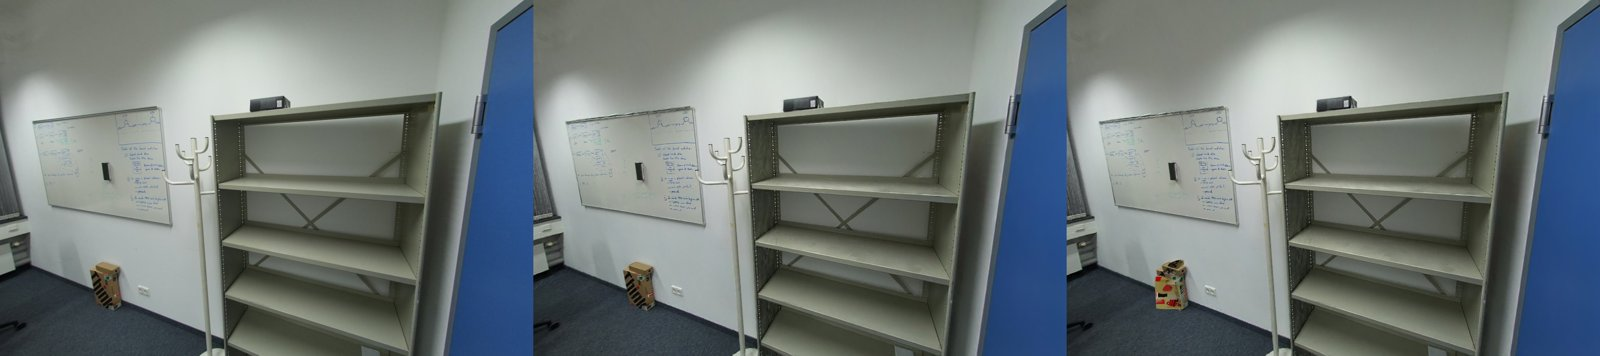
\includegraphics[width=\linewidth]{figs/eval_strip.jpg}
\caption{Photo (left), SceneSplat background render (middle), and \name\
composite twin (right) on a validation scene.}
\label{fig:teaser}
\end{figure}

\subsection{Main Results: GT-Driven vs Fully Automatic}
\begin{table}[t]
\caption{All 50 ScanNet++ validation scenes.}
\label{tab:main}
\centering\small
\begin{tabular}{lcc}
\toprule
 & GT-driven & Automatic (no GT) \\
\midrule
instances & 789 & 1{,}082 \\
yield (tier A+B) & 57.9\% (76\%$^\dagger$) & 62.0\% \\
geometry F1@20mm & 0.783$^{\mathsection}$ & 0.582$^\ddagger$ \\
drop-test stable (SR) & 77.2\% & 75.4\% \\
per scene / object & 11.6 min / 44 s & 17.0 min / 47 s \\
\bottomrule
\end{tabular}\\[2pt]
{\footnotesize $^\dagger$excluding one library outlier (200 shelved
books, 189 correctly rejected). $^{\mathsection}$hybrid generation
(Sec.~\ref{sec:exp-gen}); 0.708 single-view-only. $^\ddagger$single-view
only, scored against the vertex-IoU-matched GT instance (381 of 671 A+B
objects match at IoU$\geq$0.25; scoring against the discovered
instance's own extraction, the only option without annotations, reads
0.630); the automatic mode's discovery prompts cover fewer categories
than the GT whitelist (Sec.~\ref{sec:discovery}), so its 1{,}082
instances are not a superset of the 789.}
\end{table}

Table~\ref{tab:main}: removing all annotations costs little in yield
and stability, at $\sim$1.5$\times$ the runtime (discovery replaces
free GT segments). Geometry is where autonomy is paid for: like-for-like
(single-view generation, matched-GT scoring) F1@20mm drops from 0.708
to 0.582, and discovery recovers 336 of 844 whitelist-sized GT
instances while proposing 522 further instances outside the matched
set (extra categories, duplicates, and hallucinations share that
count). On the official DSLR test split---views the background splat
never trained on---the composite twin scores 28.32\,dB vs the
SceneSplat background's 28.89 (SSIM 0.906/0.909), a 0.57\,dB gap; the
fully automatic twin scores 27.52\,dB.\footnote{Not comparable to the
background PSNR reported by~\cite{simfoundry} (15.29\,dB): that protocol
scores renders against a real video of the physically cleared room, while
ours is novel-view synthesis against held-out frames of the official test
split.} That composite still contains
the original objects; on the four scenes with a completed
removal-and-fill background, compositing assets onto the \emph{clean}
background recovers most of the removal cost (pilot scene: 28.39\,dB vs
27.55 clean-only and 29.59 raw-composite), which is the configuration
that stays photorealistic once objects move.

\ifextended
\subsection{Where the Yield Goes: Per-Category Results}
\label{sec:exp-cat}
\begin{table}[t]
\caption{Per-category breakdown, GT-driven mode, all 50 scenes. Yield is
tier A+B; F1@20 is pooled over tier-A+B objects; \emph{stable} is the
corrected link-frame drop test.}
\label{tab:percat}
\centering\small
% generated by simany.eval.make_paper_tables -- do not edit
\begin{tabular}{lrrrr}
\toprule
category & $n$ & yield & F1@20 & stable \\
\midrule
book & 253 & 21\% & 0.809 & 87\% \\
box & 135 & 76\% & 0.548 & 68\% \\
bottle & 78 & 51\% & 0.763 & 62\% \\
keyboard & 39 & 97\% & 0.898 & 97\% \\
cup & 38 & 68\% & 0.879 & 88\% \\
shoe & 31 & 84\% & 0.648 & 92\% \\
cardboard box & 31 & 81\% & 0.531 & 68\% \\
mouse & 28 & 96\% & 0.969 & 96\% \\
bag & 25 & 88\% & 0.525 & 64\% \\
plant pot & 16 & 75\% & 0.673 & 75\% \\
telephone & 16 & 81\% & 0.671 & 85\% \\
backpack & 11 & 91\% & 0.433 & 20\% \\
jar & 11 & 18\% & 0.711 & 100\% \\
speaker & 10 & 50\% & 0.673 & 80\% \\
plate & 10 & 90\% & 0.827 & 67\% \\
\midrule
other (15 categories) & 57 & 79\% & 0.775 & 80\% \\
\midrule
all & 789 & 58\% & 0.708 & 77\% \\
\bottomrule
\end{tabular}

\end{table}

Aggregates hide a wide spread (Table~\ref{tab:percat}). Rigid, opaque,
well-observed desk objects are essentially solved: mouse (F1 0.969, 96\%
yield), keyboard (0.898, 97\%), cup (0.879), plate (0.827). The hard
categories are hard for two distinct reasons, and conflating them would be
a mistake.

\emph{Low yield, high F1} --- books (21\% yield but F1 0.809 on those that
pass) and jars (18\%, 0.711). These are dominated by the library scene's
shelved books, which are mutually occluded and rarely admit a usable
best view; the ones that do pass register well. The bottleneck is
\emph{observation}, not generation.

\emph{High yield, low F1} --- bags (88\% yield, F1 0.525), backpacks (91\%,
0.433), cardboard boxes (81\%, 0.531), boxes (76\%, 0.548). These are
deformable or near-deformable objects that we treat as rigid, and large
objects whose unobserved back faces the generator must invent. The
bottleneck is \emph{representation}. Notably these are also the
categories where multi-view generation helps most
(Sec.~\ref{sec:exp-gen}), which is consistent with the diagnosis.

Bottles sit apart: 51\% yield at F1 0.763, with the loss concentrated in
transparency rather than in either mechanism above.
\fi

\conf{Per-category results (extended version) show the aggregate hides a
wide spread: mouse and keyboard exceed F1 0.89 at $>$95\% yield, while bags
and backpacks reach 0.53/0.43 despite $\approx$90\% yield, and books yield
only 21\% but score 0.809 when they do pass---observation-limited and
representation-limited failures are distinct.}


\subsection{Ablation Ladder: How Much Ground Truth Is Needed}
\label{sec:ladder}
Table~\ref{tab:main} removes semantic annotations but still relies on
ScanNet++'s own high-fidelity scan mesh for raycasting, registration,
and the physics-collision background. We extend the ladder one rung at
a time to isolate exactly which piece of ``ground truth'' the pipeline
actually needs: (B) automatic segmentation with the dataset mesh
(Table~\ref{tab:main}'s automatic column); (C) a mesh substitute derived
from nothing but the trained splat itself, via depth rendered at every
third training view and fused by TSDF integration (voxel 5\,mm,
truncation 2\,cm, alpha cut-off 0.6, following 2DGS's extraction
convention~\cite{twodgs})---evaluated both under GT segments
(C\textsubscript{GT}, isolating the mesh swap against row A) and under
automatic segmentation (C\textsubscript{SAM3}, against row B); and (D)
the single-image zero-shot mode, which additionally drops multi-frame
discovery and the reconstructed mesh entirely, relying on monocular
metric depth from one representative frame. Rows A, C\textsubscript{GT},
and D score registered assets against independent GT instance geometry;
rows whose instances are self-discovered (B, C\textsubscript{SAM3})
additionally require matching each discovered instance to its GT
counterpart before scoring, and we report both the matched-GT score and
the own-extraction score the pipeline can compute without annotations.
All rungs use single-view generation, so row A here reads 0.708, not
Table~\ref{tab:main}'s hybrid 0.783.

\begin{table}[t]
\caption{Ablation ladder, all 50 ScanNet++ validation scenes.}
\label{tab:ladder}
\centering\small\setlength{\tabcolsep}{4pt}
\begin{tabular}{@{}lccc@{}}
\toprule
 & inst./scenes & yield & F1@20mm \\
\midrule
A: GT seg.\ + GT mesh & 789/50 & 58.0\% & 0.708 \\
B: SAM3 + GT mesh & 1{,}082/50 & 62.0\% & 0.582$^\ddagger$ \\
C$_{\text{GT}}$: GT seg.\ + derived mesh & 678/49$^\dagger$ & 56.0\% & 0.693 \\
C$_{\text{SAM3}}$: SAM3 + derived & 930/49$^\dagger$ & 59.0\% & 0.553$^\P$ \\
D: single-image zero-shot & 389/40$^\dagger$ & 17.2\% & 0.309 \\
\bottomrule
\end{tabular}\\[2pt]
{\footnotesize Pooled F1 over tier-A+B objects, single-view generation.
$^\ddagger$vs matched GT instances (381/671 match; 0.630 vs own
extraction). $^\P$vs matched GT instances (421/930 discovered instances
match; 240 of these are tier A+B; 0.667 vs own extraction, 549 objects).
$^\dagger$scenes contributing $\geq$1 instance, of
50. Row C$_{\text{GT}}$: one scene crashed in mask lifting (fixed); one
scene's mesh fusion needed a higher-memory retry. Row C$_{\text{SAM3}}$:
same fixes plus an auto-dispatch bug.
Row D: 5 scenes contain no object of its 7 target categories, 2 hit a
generator crash on a degenerate crop, 3 completed with no SAM3
detection in the chosen frame; 2 further scenes crashed after scoring
and their 4 (all rejected) instances are included. Row D's F1 covers
its 67 A+B objects; pooling over all 167 GT-matched non-rejected
objects gives 0.128.}
\end{table}

The result (Table~\ref{tab:ladder}) is not what a ``ground truth vs.\
none'' framing would predict. Under GT segments, swapping the dataset's
laser-scan mesh for one fused purely from the splat's own rendered depth
costs 2 points of yield and 0.015 F1 (row C$_{\text{GT}}$ vs.\ row A:
0.693 vs.\ 0.708); under automatic segmentation the same swap costs 3
points of yield and, on the trustworthy matched-GT score, 0.029 F1 (row
C$_{\text{SAM3}}$ vs.\ row B: 0.553 vs.\ 0.582)---own-extraction scoring
alone would have read this backwards (0.667 vs.\ 0.630), since it
credits the derived-mesh pipeline against its own discovered instances
rather than an independent reference. Either way the derived mesh is
nearly as usable for raycasting, registration, and collision as the
dedicated scan---small, consistent costs, not a cliff.

The real cliff is row D: dropping the reconstruction itself (mesh
\emph{and} multi-view discovery, down to one image and monocular depth)
collapses yield to 17.2\%---even the assets that do register well (F1
0.309 over the surviving 15\%) are too few to furnish a twin. The
dataset's own mesh, in other words, was never load-bearing---\emph{having
a reconstruction at all} is. This is the practical takeaway for anyone
wanting to apply the method outside a scan dataset: a phone video plus
off-the-shelf SfM and splat training suffices; a single photograph does
not.

\subsection{Instance Discovery vs MaskClustering}
\label{sec:exp-disc}
\begin{table}[t]
\caption{Discovery with the same SAM3 mask generator (pilot scene).}
\label{tab:mc}
\centering\small
\begin{tabular}{lccc}
\toprule
F1 & frames & IoU@0.25 & IoU@0.5 \\
\midrule
MaskClustering (native density) & 164 & 0.321 & 0.107 \\
MaskClustering (matched budget) & 28 & 0.571 & 0.286 \\
\textbf{\name\ (ours)} & 28 & \textbf{0.605} & \textbf{0.419} \\
\bottomrule
\end{tabular}
\end{table}
Both methods consume masks from the same SAM3 model, prompts, and
threshold, isolating the 3D aggregation up to frame density; because
MaskClustering's own protocol ingests every other frame while our
pipeline strides every 12th, we report it at both densities
(Table~\ref{tab:mc}). The comparison is instructive: at its native
density MaskClustering over-segments badly (38 predictions for 18 GT
objects), but this is largely a density artifact---at our 28-frame
budget it produces 17 predictions and closes most of the gap at the
loose threshold (0.571 vs.\ our 0.605 at IoU\,0.25). What survives
density matching is localization precision: at IoU\,0.5 our
occlusion-aware mesh lifting keeps a $1.5\times$ F1 edge (0.419 vs.\
0.286). We attribute the difference to the dominant-depth cluster filter
and the first-hit visibility test, both of which reject the silhouette
spill-over that a view-consensus graph has no geometric means to detect.
MaskClustering runs with its released ScanNet++ hyperparameters, which
were tuned for Cropformer masks; we did not re-tune them for SAM3. This is
a single-scene benchmark.

\subsection{Single- vs Multi-View Generation}
\label{sec:exp-gen}
\ifextended
\begin{table}[t]
\caption{Residual-gated hybrid over all 50 scenes: mean F1@20\,mm of each
generator, the fraction of objects for which the chamfer gate selected
multi-view, and the number of multi-view collapses (F1$<$0.1). Categories
with $\geq4$ dual-scored objects.}
\label{tab:hybridcat}
\centering\scriptsize
% generated by simany.eval.make_paper_tables -- do not edit
\begin{tabular}{lrrrrr}
\toprule
category & $n$ & TRELLIS & RVG & RVG chosen & collapses \\
\midrule
box & 103 & 0.548 & 0.572 & 56\% & 5 \\
book & 53 & 0.813 & 0.806 & 47\% & 3 \\
bottle & 40 & 0.763 & 0.665 & 45\% & 6 \\
keyboard & 37 & 0.896 & 0.907 & 57\% & 0 \\
mouse & 27 & 0.969 & 0.979 & 81\% & 0 \\
cup & 26 & 0.879 & 0.825 & 31\% & 1 \\
cardboard box & 25 & 0.531 & 0.674 & 68\% & 0 \\
shoe & 24 & 0.648 & 0.687 & 50\% & 0 \\
bag & 22 & 0.525 & 0.579 & 45\% & 1 \\
telephone & 13 & 0.671 & 0.776 & 38\% & 0 \\
plant pot & 12 & 0.673 & 0.707 & 42\% & 0 \\
backpack & 10 & 0.433 & 0.538 & 80\% & 0 \\
plate & 9 & 0.827 & 0.870 & 56\% & 0 \\
laptop & 7 & 0.771 & 0.846 & 57\% & 0 \\
speaker & 5 & 0.673 & 0.310 & 20\% & 2 \\
kettle & 5 & 0.654 & 0.674 & 60\% & 0 \\
basket & 5 & 0.587 & 0.533 & 80\% & 0 \\
pen & 4 & 0.998 & 1.000 & 75\% & 0 \\
headphones & 4 & 0.776 & 0.741 & 50\% & 0 \\
\midrule
all & 453 & 0.708 & 0.719 & 54\% & 18 \\
\bottomrule
\end{tabular}

\end{table}
\fi


Multi-view reconstruction-consistent generation tends to win on
well-observed opaque objects and to collapse on transparency---but not
uniformly.\ext{ Table~\ref{tab:hybridcat} shows the pattern across all 453
dual-scored objects.} The two generators are nearly tied on average
(0.708 vs.\ 0.719), which is precisely why a per-object gate rather than a
global choice is the right structure: the mean hides that multi-view wins
by $+0.14$ on cardboard boxes and $+0.11$ on backpacks while losing by
$-0.36$ on speakers and $-0.10$ on bottles. Even within one category the
regimes coexist---on the pilot scene's five identical-label bottles, three
multi-view reconstructions collapse outright (F1 0.007--0.045) and two
\emph{beat} single-view (0.95/0.90).

The residual-selected hybrid resolves this per object. Across the 457
non-rejected objects it lifts pooled F1@20\,mm from 0.708 (single-view
only) to \textbf{0.783}, choosing the multi-view asset for 54\% of them.
Critically, the multi-view generator collapsed on 18 objects and the
chamfer gate caught \emph{all 18}, falling back to single-view without any
category knowledge. Dataset-wide the gate disagrees with the F1-optimal
choice on 64 of 453 dual-scored objects (14.1\%, worst case $-0.31$ F1,
mean $-0.04$), yet its pooled F1 is within \textbf{0.006} of the oracle
hybrid that always picks the better asset (0.783 vs.\ 0.789)---most
disagreements are near-ties. The dual-generate-and-select stage costs
54\,s per object (6.8 A6000-hours for the full benchmark). We use TRELLIS
v1; a newer release claims explicit transparency support, which would
likely change the balance of this table.

\subsection{Removal and Verification}
\begin{figure}[t]
\centering
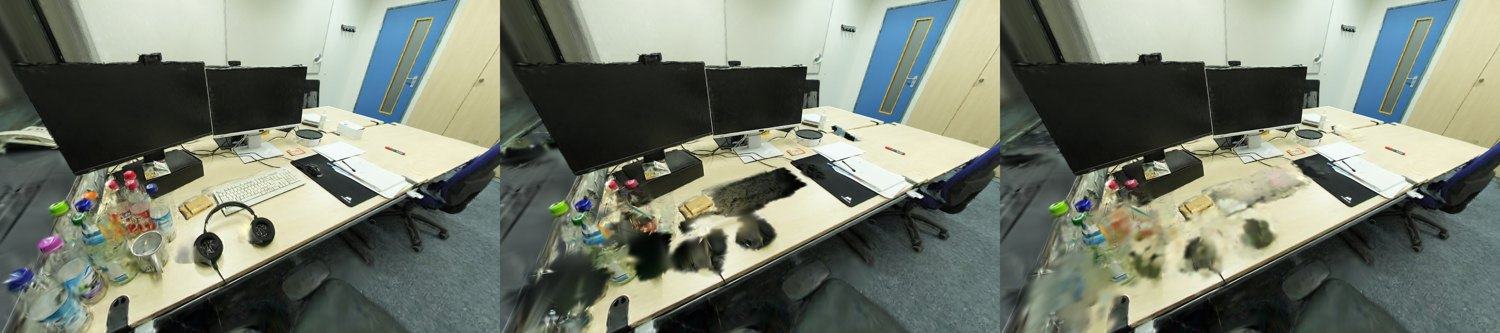
\includegraphics[width=\linewidth]{figs/cmp_bottles_v3.jpg}
\caption{Original splat / after removal / after support-plane filling on
the hardest case (transparent bottle cluster).}
\label{fig:removal}
\end{figure}
\ifextended
\begin{figure}[t]
\centering
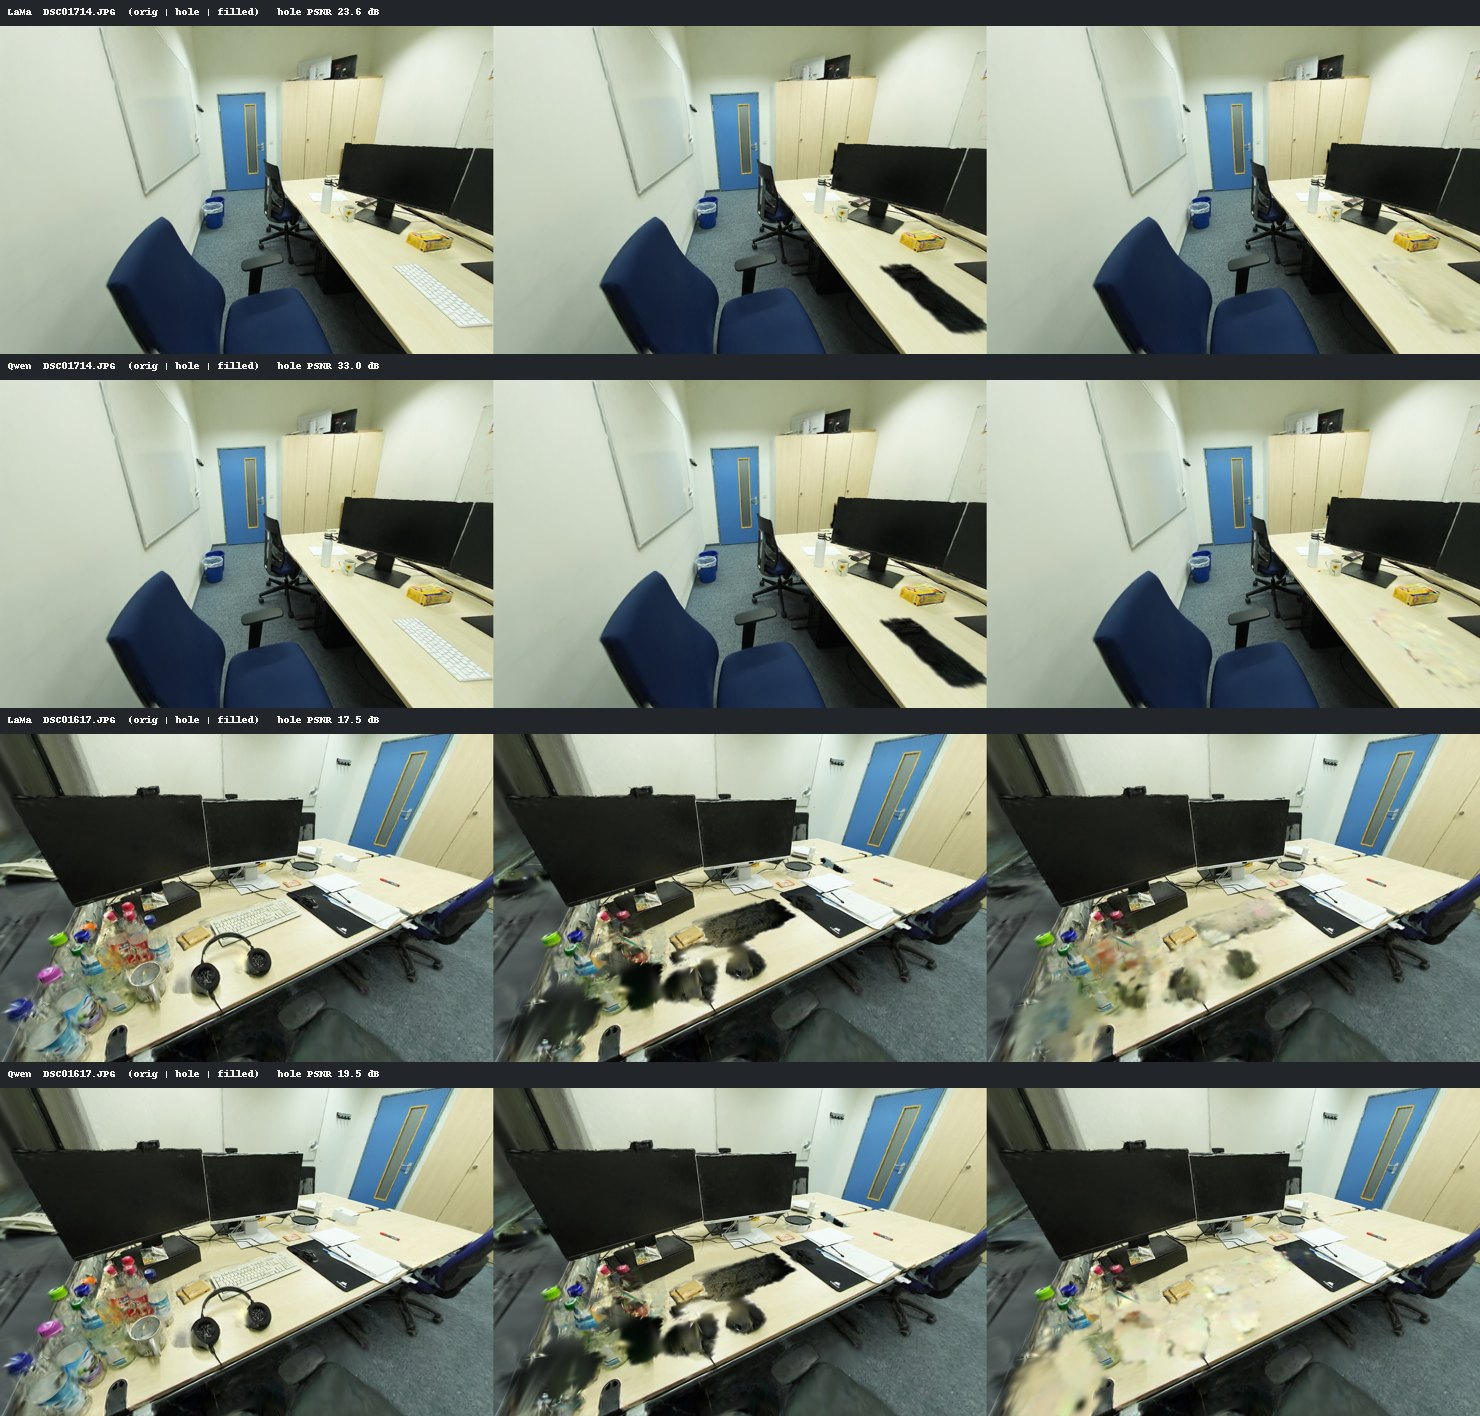
\includegraphics[width=\linewidth]{figs/qwen_vs_lama.jpg}
\caption{Inpainting backend as fill supervisor. Qwen-Image-Edit
decisively wins on flat structured surfaces; elsewhere the two are
comparable with large per-frame variance.}
\label{fig:qwenlama}
\end{figure}
\fi

On the pilot scene (16 objects; the battery has not yet been run at
fleet scale) the verification battery reports: alpha coverage $>0.95$
for 14/16 objects---the two exceptions are cardboard boxes (0.83/0.86)
whose box-scale holes exceed the support-plane fill's design scale, the
same failure mode that keeps furniture out of the main protocol
(Sec.~\ref{sec:furniture}); support residuals of 12--26\,mm for small
opaque objects vs 32--111\,mm for bottles (and up to 0.8\,m for the
boxes); residual re-detection passes 14/16 objects, both failures
transparent bottles (residual scores 0.27/0.36 vs 0.91/0.93 before
removal). That the battery independently rediscovers the two failure
classes the rest of the paper identifies---transparency and
scale---without consulting any annotation is the point of building it.

FlashSplat's optimal mask-assignment~\cite{flashsplat}, adapted to
object-centric view sets, agrees with our final removal set at union IoU
0.649 (recall 0.87 of our set); per-object disagreement correlates with
object size and thin geometry (mice, keyboards) as much as with
transparency, so we read it as two defensible selection conventions rather
than an error in either. As the fill supervisor, Qwen-Image-Edit
decisively beats LaMa on the flat structured keyboard-desk surfaces (mean
hole PSNR 34.3 vs 23.9\,dB over the six supervision frames); over the
remaining 25 frames the two are comparable (19.4 vs 20.5\,dB, LaMa
slightly ahead) with large per-frame variance in both directions\ext{
(Fig.~\ref{fig:qwenlama})}.

\subsection{Physical Plausibility}
\label{sec:exp-phys}
\ifextended
\begin{figure}[t]
\centering
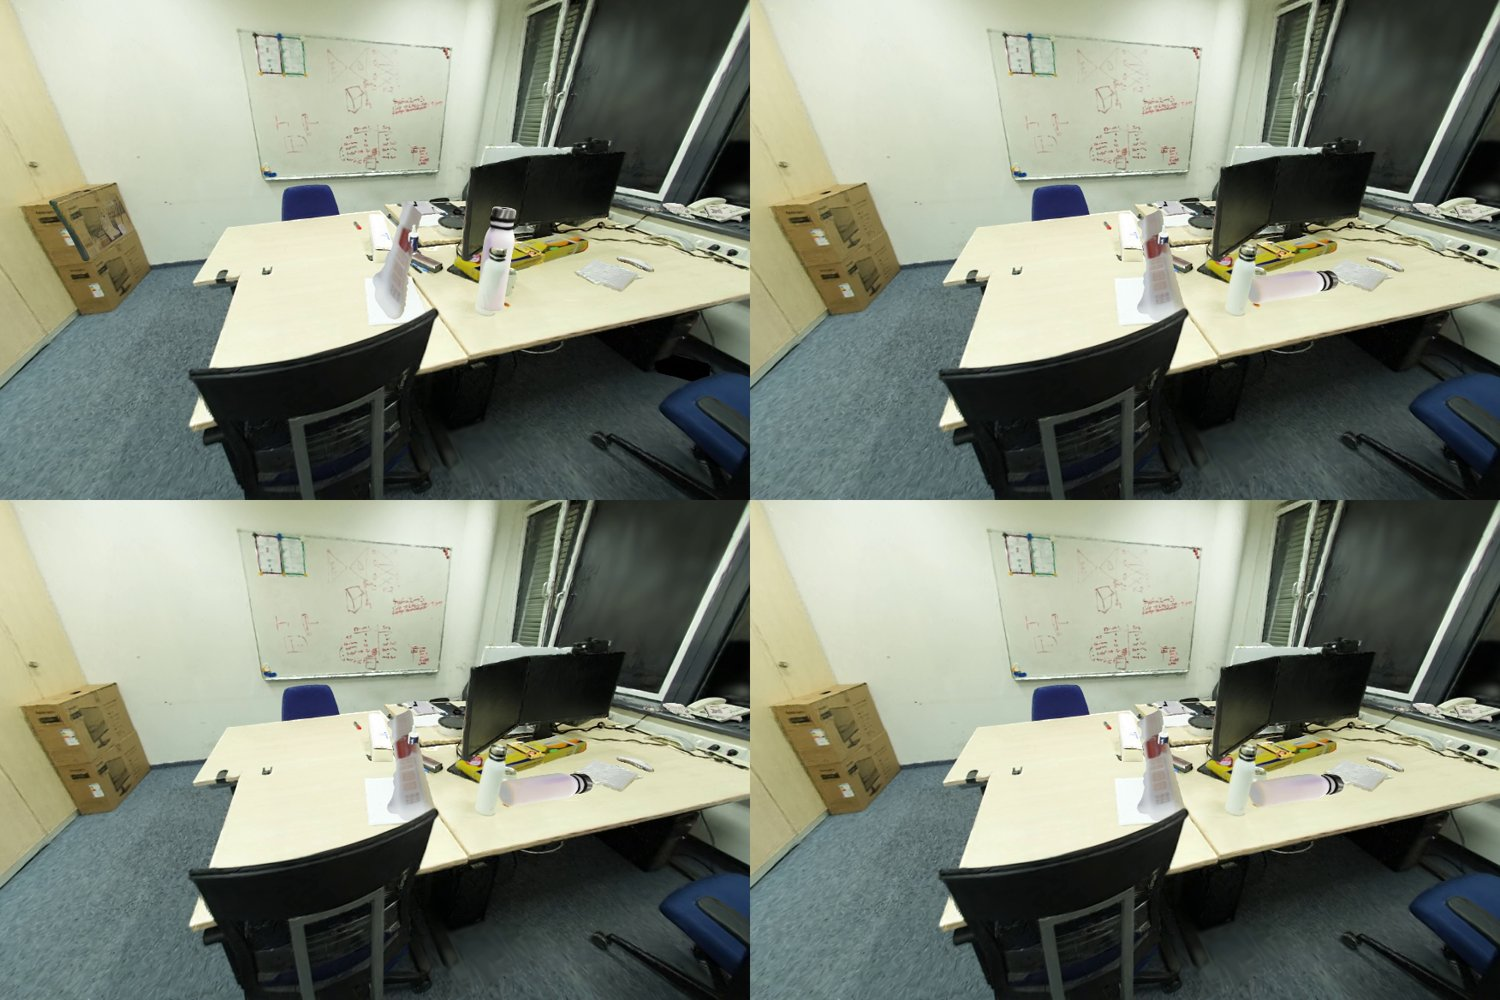
\includegraphics[width=\linewidth]{figs/mj_photoreal_grid.jpg}
\caption{Exported MJCF scenes stepped in MuJoCo and rendered by
compositing the asset Gaussians at the simulator's object states.}
\label{fig:mujoco}
\end{figure}
\fi

\begin{table}[t]
\caption{Stability ratio vs.\ the drift threshold. The 3\,cm column is the
headline number; p50/p90 are the drift distribution's percentiles.}
\label{tab:srsweep}
\centering\small
% generated by simany.eval.make_paper_tables -- do not edit
\begin{tabular}{lrrrrrrr}
\toprule
mode & $n$ & 1\,cm & 2\,cm & 3\,cm & 5\,cm & 10\,cm & drift p50 / p90 \\
\midrule
GT-driven & 457 & 71.3 & 74.2 & 77.2 & 79.9 & 86.9 & 0.03 / 138\,mm \\
automatic & 671 & 70.5 & 73.8 & 75.4 & 78.7 & 84.6 & 0.02 / 157\,mm \\
\bottomrule
\end{tabular}

\end{table}

Under the protocol of Sec.~\ref{sec:setup}, \name\ reaches an SR of
\textbf{77.2\%} (GT-driven) and 75.4\% (automatic). For context,
PhyRecon~\cite{phyrecon} reports 78.16\% on ScanNet++ under an Isaac Gym
drop test, against 26.43\% (RICO) and 25.28\% (ObjectSDF++);
HoloScene~\cite{holoscene} reports 93.9\% under an Isaac Sim protocol in
which the same ObjectSDF++ baseline instead scores 81.6\%. These numbers
are \emph{not} directly comparable---simulator, drift threshold and
duration all differ, and the two published protocols disagree by over 50
points on a shared baseline.

Table~\ref{tab:srsweep} is our response to that: rather than defend one
threshold, we publish the curve. The important observation is that it is
\emph{flat}. Moving the criterion from 1\,cm to 5\,cm---a $5\times$
relaxation---moves SR by only 8.6 points (71.3 to 79.9), and the drift
distribution explains why: the median object moves 0.03\,mm while the 90th
percentile moves 138\,mm. Stability is bimodal. Objects either settle
essentially exactly where they were placed, or they fall over and travel
far. Almost nothing sits near the threshold, so the choice of criterion is
not what separates these systems, and a 50-point gap between two published
protocols cannot be a thresholding artifact either. It follows that the
frame convention, the simulator's contact model, and the asset population
are the variables that matter --- which is an argument for reporting all
three, not for standardizing on a number.

Two further observations. First, the COM-versus-link frame convention
reclassifies only 3 of 457 objects here, so while it must be stated it is
not the reason different papers disagree. Second, and less comfortably for
us: the residual-gated hybrid that \emph{raises} geometry F1 from 0.708 to
0.783 slightly \emph{lowers} stability, from 79.9\% to 76.6\% with the
frame convention held fixed. Better surface geometry is not the same thing
as better physical behaviour---the multi-view assets are more faithful and
more detailed, and detail includes the small irregular contact patches
that make an object tip. We report both directions rather than choosing
the flattering one.

The dominant residual failure is not asset geometry but support modelling:
the MJCF export approximates the background with per-object static slabs
rather than the full scan mesh, so an object that drifts a few centimetres
can slide off its own slab, whereas the PyBullet export, which collides
against the carved scan, does not exhibit this.
\ext{Fig.~\ref{fig:mujoco} shows exported scenes stepped in MuJoCo and
rendered through the composited asset Gaussians.}

\subsection{Preliminary Extension to Furniture}
\label{sec:furniture}
The pipeline is vocabulary-agnostic: enabling a 45-alias furniture
whitelist tier on the pilot scene (a single-scene probe, GT-driven)
yields 39 instances at 82\% tier-A+B (monitors 5A+1B with F1 up to
0.79, office chairs 4/4, trash cans 0.83--0.91).
Two gaps keep furniture out of our main protocol: large
partially-observed desks defeat single-view generation, and
furniture-scale removal leaves holes one to two orders of magnitude
larger than the support-plane fill was designed for, producing visible
residue in the edited splat. We therefore report all benchmark numbers
on the manipulable-object vocabulary and leave furniture as an opt-in
extension.

\subsection{Efficiency}
\ifextended
\begin{table}[t]
\caption{Where the 9.68 A6000-hours go (GT-driven, 50 scenes).}
\label{tab:timing}
\centering\small
% generated by simany.eval.make_paper_tables -- do not edit
\begin{tabular}{lrr}
\toprule
stage & A6000-h & share \\
\midrule
registration & 3.87 & 40\% \\
collision + physics + URDF & 2.73 & 28\% \\
asset generation (TRELLIS) & 2.20 & 23\% \\
instance enumeration + best-view crop & 0.46 & 5\% \\
SAM3 mask evidence & 0.22 & 2\% \\
render metrics & 0.20 & 2\% \\
drop test + report & 0.01 & 0\% \\
\midrule
total & 9.68 & 100\% \\
\bottomrule
\end{tabular}

\end{table}
\fi


Small-object tier, counting every GPU-second including resumed partial
runs: GT-driven 9.7 A6000-hours for 50 scenes (11.6\,min/scene), fully
automatic 14.1 A6000-hours (17.0\,min/scene; discovery replaces free GT
segments and registration targets are noisier). Extrapolating linearly to
all 1{,}018 ScanNet++ scenes: $\approx$197 (GT-driven) / $\approx$288
(automatic) A6000-hours.

\ext{Table~\ref{tab:timing} }\conf{A stage breakdown }is worth
noting because it is the opposite of what the pipeline's description
suggests. Generation---the stage with a large diffusion model in it---is
23\% of the budget at roughly 10\,s per object. The expensive stages are
\emph{registration} (40\%) and \emph{convex decomposition} (28\%), both of
which are classical CPU-bound geometry running on 20k-point clouds and
40k-triangle meshes. A practical consequence: this pipeline is not
GPU-bound, and the obvious speedups are a coarser yaw grid or a cheaper
decomposition budget, not a smaller generator.

HoloScene~\cite{holoscene} reports 8.3\,h per scene ($43\times$ /
$29\times$ our two modes; we could not confirm its exact GPU model, so
the multiplier is indicative). SimFoundry~\cite{simfoundry} reports
19.98--67.13\,min per scene at $\approx$5\,min per object on an RTX 3090,
i.e.\ $\approx6.5\times$ our per-object cost across different hardware,
plus a further $\approx$90\,min per scene if its automatic background
route is used.

\subsection{Task-Level Validation Feasibility}
\label{sec:behavior1k}
Geometry and photometric metrics do not establish that a twin supports
household \emph{activity}. BEHAVIOR-1K~\cite{behavior1k} would be a
natural task-level validator, but its 50 scenes are artist-built assets,
not real scans, so \name\ cannot run on them. We instead ask the inverse
question---how many BEHAVIOR-1K activities could be grounded \emph{in a
\name\ twin}---by strictly intersecting each activity's required
rigid-body categories against our vocabulary and against the labels we
have actually discovered across the 50 scenes. Of 1,015 activities with
at least one rigid-object requirement, 75\% specify rooms a scan dataset
would plausibly contain, 2.3\% are vocabulary-complete, and 0.6\% (six
kitchen/utility activities) are fully groundable in objects we have
already generated; mean per-activity coverage is 24.9\% (vocabulary) and
9.8\% (discovered). This is a static feasibility check, not a simulator
run: a genuine but narrow beachhead, quantifying how much vocabulary
expansion would close the gap.\ext{ Appendix~\ref{app:behavior} gives the
matching protocol.}

%======================================================================
\ifextended
\section{Discussion}

\textbf{What the ablation ladder generalizes to.} The finding that a
splat-derived mesh substitutes for a laser scan at a cost of 0.015 F1 is
the result with the widest reach, because it decouples the method from
scan datasets. Together with row D it delimits the operating regime
precisely: the pipeline needs multi-view coverage and a metric
reconstruction, and is indifferent to how good that reconstruction is
within a broad band. It does not need annotations, and it does not need a
survey-grade scanner.

\textbf{Geometry and physics are not the same objective.} The hybrid
result and the stability result point in opposite directions
(Sec.~\ref{sec:exp-phys}), and we think this is general rather than an
artifact. Surface-accuracy metrics reward detail; rigid-body stability
rewards flat, convex, well-supported bases. A pipeline optimized purely on
F1 will drift toward assets that simulate worse. This argues for reporting
both, and eventually for a selection gate that scores candidates on
simulated behaviour as well as on registration residual---a
straightforward extension of the residual gate we already have, since the
drop test costs milliseconds.

\textbf{Verification is cheap and should be standard.} The battery costs a
few seconds per object and needs no annotation, and it independently
recovered both of the failure classes we found by other means. Its real
value is operational: at 1{,}000 instances per 50 scenes, no one inspects
outputs by hand, and a system without self-scoring degrades silently as it
scales.

\textbf{What we would do differently.} Registration and convex
decomposition consume 68\% of the compute for stages that are, in
principle, cheap; both were written for correctness and never optimized.
And the automatic mode's prompt vocabulary, not its geometry, is what
bounds BEHAVIOR-1K coverage at 2.3\%---the cheapest available improvement
to task-level usefulness is a larger prompt set, not a better generator.
\fi


%======================================================================
\section{Limitations}
\name\ requires a reconstruction (mesh and splat) rather than raw video;
transparent objects remain hardest for both removal and multi-view
generation, and box-scale removal holes exceed the support-plane fill's
design scale; articulation is not modeled and deformables are treated
as rigid. Articulation recovery is an orthogonal and actively-solved
sub-problem---from images~\cite{urdformer}, by VLM program
synthesis~\cite{articulateanything}, without annotation from point-cloud
motion~\cite{autourdf}, and natively in Gaussians~\cite{artgs}---and
composes with our pipeline, as \cite{simfoundry} does with a dedicated
articulation module.
Lighting is baked into the splats, so moved objects cast no shadows;
recovering engine-native parametric lights is the target of concurrent
work~\cite{lumera}, whose reported light-detection F1 of 0.209 at 0.5\,m
and $\approx$2.7$\times$ intensity error indicate the problem is far from
solved.
The MJCF export approximates the scene background with
per-object static support slabs rather than the full scan mesh (the
PyBullet export does collide against the carved scan), so cross-object
and object--room interactions differ between the two exports. The
registration optimizer's robustness claims (Sec.~\ref{sec:registration})
were validated on the zero-shot partial-cloud path; the benchmark
numbers register against complete instance submeshes, a better-
conditioned setting. The verification battery and the
MaskClustering/FlashSplat baselines have so far been run on one pilot
scene. Sim-to-real policy correlation is cited from~\cite{simfoundry}
rather than re-validated on hardware, and was measured there on
\emph{tabletop} twins, so it transfers to room-scale scanned scenes only
as an indication; and ScanNet++ licensing prevents redistributing the
generated assets.

\section{Conclusion}
\name\ shows that a fully automatic, annotation-free system can turn
reconstructions of real scenes into verified, editable, sim-ready
digital twins at dataset scale and interactive cost. We believe the
combination of dual-use instance discovery, transparency-robust
Gaussian editing, and supervision-independent verification is a
practical recipe for scaling real-to-sim to every scanned scene, and we
release the pipeline, benchmark protocol, and per-scene results.
